\documentclass[title-style=modern,plantuml=true,print-ndn=false,auto-generate=false,bib-file=content/literature.bib]{udhbwvst}

\dhbwSetup{%
    author          = Adrian Stengle und Simon E\ss{linger},
    faculty         = Wirtschaft,
    field of study  = Wirtschaftsinformatik,
    academic year   = 2017,
    course          = B,
    title           = Projekt Maschinenbau,
    subtitle        = Softwarekonzept,
    text type       = Seminararbeit,
    company name    = Gruppe 1 \cdot\ Animal Abduction Crew,
    lecturer        = Prof.\ Dr.\ Wolfgang Funk
}

\usepackage{booktabs} % pretty tables

\DeclareAcronym{AAR}{%
    short		= AAR,
    long		= Animal Abduction Robot
}

\DeclareAcronym{AAC}{%
    short		= AAC,
    long		= Animal Abduction Crew
}

\DeclareAcronym{WI}{%
    short		= WI,
    long		= Wirtschaftsinformatik
}

\DeclareAcronym{TM}{%
    short		= TM,
    long		= Technical Management
}

\DeclareAcronym{CSI}{%
    short		= CSI,
    long		= Camera Serial Interface
}

\DeclareAcronym{CNN}{%
    short		= CNN,
    long		= Convolutional Neural Network
}

\DeclareAcronym{R-CNN}{%
    short		= R-CNN,
    long		= Regions with Convolutional Neural Network features
}

\DeclareAcronym{SSD}{%
    short		= SSD,
    long		= Single Shot MultiBox Detector
}

\DeclareAcronym{YOLO}{%
    short		= YOLO,
    long		= You Only Look Once
}

\DeclareAcronym{CPU}{%
    short		= CPU,
    long		= Central Processing Unit
}

\begin{document}

\dhbwSetFrontMatter

\dhbwPrintTitle
\dhbwPrintNonDisclosureNotice
\dhbwPrintTableOfContents

\dhbwSetListMatter

\dhbwPrintListOfAcronyms
\dhbwPrintListOfFigures
\dhbwPrintListOfTables

\dhbwSetMainMatter

\section{Aufgabenstellung}

Diese Arbeit stellt das Softwarekonzept der Gruppe 1 \ac{AAC} für die Veranstaltung \enquote{Projekt Maschinenbau} vor.
Ziel dieser Veranstaltung ist es einen Roboter in Zusammenarbeit zwischen Studierenden der Studiengänge \ac{WI} und \ac{TM} zu entwickeln, welcher dazu in der Lage ist folgende Aufgabenstellung autonom zu lösen.

\subsection{Vorgaben}

\dhbwFigure{%
    caption	= Spielfeld,
    label	= fig:field,
    path	= content/assets/spielfeld.png,
    source	= Kickoff-Präsentation
}

\autoref{fig:field} zeigt die Dimensionen des Spielfelds in der Vogelperspektive, in welchem der Roboter ein vorher definiertes Plüschtier erkennen soll und dieses aus dem Spielfeld entfernen soll, wobei folgende Vorgaben eingehalten werden müssen:

\begin{itemize}
    \item Im Spielfeld befinden sich gleichzeitig 3 von 5 möglichen Stofftieren (Tiger, Katze, Elefant, Frosch und Stern).
    \item Je ein Tier steht im 1., 2., oder 3. virtuellen Drittel des Spielfelds.
    \item Alle Tiere stehen außerhalb des virtuellen Mittel-Korridors (s. \autoref{fig:field}).
    \item Das vorderste Tier hat mindestens 100 cm Abstand von der Startlinie.
    \item Das Tier im mittleren Drittel steht in einer anderen virtuellen „Spielhälfte“ als die beiden anderen Tiere.
    \item Der Roboter muss ein vorgegebenes Tier erkennen und einzeln aus dem Spielfeld (d. h. 5-35 cm Abstand zur Außenlinie) bringen (es zählt nur die Position des Tieres, nicht die des Roboters).
    \item Der Roboter muss das Tier autonom einsammeln (ohne Fernsteuerung o.Ä.).
    \item Der Roboter muss vier Durchläufe absolvieren, wobei die besten drei gewertet werden.
    \item Die Tiere sind jeweils zufällig platziert.
    \item Der Roboter muss die Durchläufe in jeweils 60 Sekunden absolvieren. Falls das Tier nach 60 Sekunden nicht aus dem Feld entfernt wurde, stehen maximal 30 weitere Sekunden zu Verfügung.
    \item Die Bauteile des Roboters dürfen in Summe maximal 70€ kosten.
    \item Die Basiskonstruktion soll primär aus gegebenen Holzstangen bestehen.
    \item Schließlich muss ein Raspberry Pi 3 B verwendet werden.
\end{itemize}

Gelistete Anforderungen wurden der Kickoff-Präsentation des Projektes entnommen.\ifootcite{kickoff}

\subsection{Materialvorgaben}

Des Weiteren ist folgende Materialliste vorgegeben:

\begin{itemize}
    \item 1 Raspberry-Pi (muss verwendet werden)
    \item 2 H-Brücken 298N zur Motorsteuerung
    \item 2 Motoren
    \item 1 Kamera (muss verwendet werden)
    \item 5 Tiere
    \item Sensoren zur Linienerkennung
    \item Stromversorgung und Ladegerät
    \item Holzstangen: 1x1 cm, 1x2 cm, 2x2 cm (müssen verwendet werden)
    \item Grundlegende Schrauben nach Bedarf
    \item Grundlegende Kabel nach Bedarf 
\end{itemize}

Auch die Materialvorgaben wurden der Kickoff-Präsentation des Projektes entnommen.\ifootcite{kickoff}

\section{Konzept}

Für die Lösung, der in \autoref{sec:task} beschriebenen Aufgabe wird eine optische Objekterkennung in Kombination mit Ultraschall- und Infrarotsensoren für die Navigation verwendet, ein Greifarm für die Fixierung eines Tieres, zwei Motoren für den Antrieb des Roboters, sowie ein Mikrofon und ein Lautsprecher für eine Sprachsteuerung herangezogen.
Aus diesem Lösungsansatz lassen sich mehrere Anforderungen, in Form von Use-Cases, an den \ac{AAR} ableiten.

\subsection{Aufbau des Roboters}
Unser Roberter trägt den Namen "animal abduction robot" zu deutsch Tier-Entführungsroboter, da es wie oben beschieben seine Aufgabe ist Tiere zu finden und zu bewegen.

Der nachfolgende Abschnitt behandelt hierbei wie der AAR aufgebaut ist und welche Sensoren und Komponenten hierbei für welche zwecke eingesetzt werden. Zudem wird im weiteren auf die Belegung der einzelnen GPIO Pins des Raspberry Pi eingegangen.
% erklärung name (aar = animal abduction robot)

\subsubsection{Skizze}

Auf dem nachfolgenden Bild sieht man den AAR von oben. Auffallend ist der größe Greifmechanismus, welcher die vordere Hälfte des AAR einnimmt. Die hintere Hälfte des AAR bist recht schmal gehalten und beinhaltet sämtliche Elektronik, wie den Akku, den Raspberry Pi, ein Breadboard und eine vielzahl an Sensoren. 

Hierbei ist zu beachten, dass sie die Ultraschallsensoren noch nicht an dem Roboter befinden, da diese nur genutzt werden, falls die Bilderkennung nicht so gut funktionieren sollte wie angenommen.
Falls sich ein Tier seitlich des AAR befinden sollte würde es eine besonders hohe Entfernung anzeigen, da die Tiere den Schall der Ultraschallsensoren schlucken würde. So können wir bestimmen ob sich dort ein Tier befindet und den AAR darauf ausrichten. 

Die Hauptbestandteile des AAR und ihre Aufgaben werden mithilfe der nachfolgenden Skizze und der unten stehenden Tabelle "Aufbau Roboter" genauer erläutert.

\dhbwFigure{%
    caption	= Animal Abduction Robot,
    label	= fig:aar,
    path	= content/assets/aar.jpg,
    source	= Eigene Darstellung
}

\begin{dhbwtable}{%
    caption	= Aufbau Roboter,
    label	= tab:show_parts_at_aar,
    source	= Eigene Darstellung,
}
    \begin{tabular}{llll}
        \toprule
        \textbf{Nummer}     & \textbf{Bauteil}      &\textbf{Beschreibung}   \\\midrule
        1   	            & Akku                  & Stromversorgung für Motoren und Raspberry Pi\\
        2                   & Raspberry Pi          & Recheneinheit und Ansteuerungsmodul \\
        3                   & Ultraschallsensor rechts   & Erkennung falls sich ein Tier Rechts des AAR befindet  \\
        4                   & Ultraschallsensor links   & Erkennung falls sich ein Tier Links des AAR befindet  \\
        5                   & H-Brücke für den Greifer   & Steuert die Motoren für den Greifer an   \\
        6                   & H-Brücke für den Antrieb   & Steuert die Motoren des Antriebes an   \\
        7                   & Spannungswandler   & regelt die Spannung des Akkus für den Raspberry auf 5 Volt runter  \\
        8                   & Motor+Getriebe Greifer rechts   & bewegt den rechten Teil des Greifarms  \\
        9                   & Motor+Getriebe Greifer links   & bewegt den linken Teil des Greifarms  \\
        10                  & Infrarot links   & erkennt eine Linie auf der linken Seite  \\
        11                  & Infrarot rechts   & erkennt eine Linie auf der rechten Seite  \\
        12                  & Infrarot mitte   & erkennt ob sich ein Tier vor dem AAR befindet  \\
        13                  & Kamera   & wird für die Objekterkennung genutzt  \\
        14                  & Antriebsmotor rechts   & dreht das rechte Rad  \\
        15                  & Antriebsmotor links   & dreht das linke Rad  \\\bottomrule
    \end{tabular}    
\end{dhbwtable}




% bild
% nennung und beschreibung der komponenten
% warum diese komponenten?; ultraschall-geschichte...

\subsubsection{Schaltplan}
Da wir durch den Greifmechanismus und die Notlösung mit hilfe der Ultraschallsensor einen relativ hohe Anzahl an Komponenten besitzen, welche angesteuert oder ausgelesen werden müssen, ist es für uns besonders wichtig einen Überblick zu haben, wie die Sensoren miteinander angeschlossen sind und an welchen GPIO Pins sich die Ein- und Ausgange befinden.

In \autoref{app:wiring_diagram} ist ein Schaltplan zu sehen, welches die Verkabelung aller Komponenten, über ein Breadboard mit dem Raspberry Pi darstellt.

\begin{dhbwtable}{%
    caption	= Belegung der GPIO Pins,
    label	= tab:gpio_pins,
    source	= Eigene Darstellung,
}
    \begin{tabular}{llll}
        \toprule
        \textbf{Bauteil}    & \textbf{GPIO Pin}     &\textbf{Funktion}   \\\midrule
        Motor rechts   	    & 18                    & Fahrtrichtung vorwärts\\
                            & 15                    & Fahrtrichtung rückwärts \\
                            & 14(PWM)               & einstellung der Geschwindigkeit\\
        Motor links   	    & 7                     & Fahrtrichtung vorwärts\\
                            & 1                     & Fahrtrichtung rückwärts \\
                            & 12(PWM)               & einstellung der Geschwindigkeit\\    
        Motoren Greifer   	& 5                     & Greifer öffnen\\
                            & 6                     & Greifer schließen \\
                            & 13(PWM)               & einstellung der Geschwindigkeit\\
        Ultraschall rechts 	& 11                    & Trigger\\
                            & 9                     & Echo \\
        Ultraschall links   & 20                    & Trigger\\
                            & 16                    & Echo \\ 
        Infrarot links      & 2                     & Input\\
        Infrarot rechts     & 3                     & Input\\
        Infrarot mitte      & 4                     & Input\\        
   \bottomrule
    \end{tabular}    
\end{dhbwtable}


% fritzing wiring diagram
\subsection{Use-Cases}\label{sec:use_cases}

Nachfolgend werden die funktionalen Anforderungen an den \ac{AAR} in Form von Use-Cases beschrieben.
Die Priorisierung erfolgt anhand einer Skala von 1 (niedrig) bis 5 (hoch).

% TODO: add detailed descriptions below the use cases

\begin{dhbwtable}{%
    caption	= Use-Case: Tier auswählen,
    label	= tab:use_case_select_animal,
    source	= Eigene Darstellung,
    float = h!
}
    \begin{tabularx}{\textwidth}{lX}
        \toprule
        \textbf{Merkmal}     & \textbf{Beschreibung}  \\\midrule
        Auslöser     & Roboter befindet sich in der Startsituation.\\
        Komponenten  & Mikrofon, Lautsprecher, Raspberry\\
        Beschreibung & Anwender spricht das Wakeword aus, gefolgt von einer Tierauswahl. Der \ac{AAR} erkennt die Auswahl und startet die Tiersuche.\\
        Priorität    & 5 \\\bottomrule
    \end{tabularx}    
\end{dhbwtable}

\begin{dhbwtable}{%
    caption	= Use-Case: Tier auffinden,
    label	= tab:use_case_find_animal,
    source	= Eigene Darstellung,
    float = h!
}
    \begin{tabularx}{\textwidth}{lX}
        \toprule
        \textbf{Merkmal}     & \textbf{Beschreibung}  \\\midrule
        Auslöser     & Tier wurde per Spracheingabe ausgewählt.\\
        Komponenten  & Kamera, Antrieb links, Antrieb rechts, Ultraschallsensor links, Ultraschallsensor rechts\\
        Beschreibung & Der \ac{AAR} fährt geradeaus durch das Spielfeld und versucht mit der Kamera das gesuchte Tier zu identifizieren und bleibt stehen, wenn das richtige Tier gefunden wurde.\\
        Priorität    & 5 \\\bottomrule
    \end{tabularx}    
\end{dhbwtable}

\begin{dhbwtable}{%
    caption	= Use-Case: Auf Tier ausrichten,
    label	= tab:use_case_turn_to_animal,
    source	= Eigene Darstellung,
    float = h!
}
    \begin{tabularx}{\textwidth}{lX}
        \toprule
        \textbf{Merkmal}     & \textbf{Beschreibung}  \\\midrule
        Auslöser     & Das gesuchte Tier wurde gefunden.\\
        Komponenten  & Kamera, Antrieb links, Antrieb rechts\\
        Beschreibung & Der \ac{AAR} dreht sich so lange, bis er direkt in Fahrtrichtung auf das gesuchte Tier ausgerichtet ist.\\
        Priorität    & 5 \\\bottomrule
    \end{tabularx}    
\end{dhbwtable}

\begin{dhbwtable}{%
    caption	= Use-Case: Zum Tier fahren,
    label	= tab:use_case_go_to_animal,
    source	= Eigene Darstellung,
    float = h!
}
    \begin{tabularx}{\textwidth}{lX}
        \toprule
        \textbf{Merkmal}     & \textbf{Beschreibung}  \\\midrule
        Auslöser     & Der \ac{AAR} ist auf das gesuchte Tier ausgerichtet.\\
        Komponenten  & Kamera, Antrieb links, Antrieb rechts, Infrarotsensor\\
        Beschreibung & Der \ac{AAR} fährt auf das erkannt Tier zu, bis der Infrarotsensor feststellt, dass das Tier direkt vor den Greifern des \acp{AAR} steht.\\
        Priorität    & 5 \\\bottomrule
    \end{tabularx}    
\end{dhbwtable}

\begin{dhbwtable}{%
    caption	= Use-Case: Tier greifen,
    label	= tab:use_case_grab_animal,
    source	= Eigene Darstellung,
    float = h!
}
    \begin{tabularx}{\textwidth}{lX}
        \toprule
        \textbf{Merkmal}     & \textbf{Beschreibung}  \\\midrule
        Auslöser     & Das gesuchte Tier befindet sich direkt vor den Greifern des \acp{AAR}. \\
        Komponenten  & Greiferantrieb links, Greiferantrieb rechts, Schließtaster \\
        Beschreibung & Der \ac{AAR} schließt den linken und rechten Greifer, bis der Schließtaster ausgelöst wird.\\
        Priorität    & 4 \\\bottomrule
    \end{tabularx}    
\end{dhbwtable}

\begin{dhbwtable}{%
    caption	= Use-Case: Tier aus dem Spielfeld fahren,
    label	= tab:use_case_move_animal,
    source	= Eigene Darstellung,
    float = h!
}
    \begin{tabularx}{\textwidth}{lX}
        \toprule
        \textbf{Merkmal}     & \textbf{Beschreibung}  \\\midrule
        Auslöser     & Das gesuchte Tier befindet sich in den geschlossenen Greifern des \acp{AAR}.\\
        Komponenten  & Antrieb links, Antrieb rechts, Liniensensor links, Liniensensor rechts\\
        Beschreibung & Der \ac{AAR} fährt geradeaus bis ein Liniensensor die Linie detektiert. Auf der Seite, auf der die Linie erkannt wurde, wird der Antrieb abgeschalten, bis der andere Liniensensor die Linie erkennt. Danach fährt der \ac{AAR} geradeaus, bis er sich mindestens 10cm von der Linie entfernt hat.\\
        Priorität    & 5 \\\bottomrule
    \end{tabularx}    
\end{dhbwtable}

\begin{dhbwtable}{%
    caption	= Use-Case: Tier loslassen,
    label	= tab:use_case_release_animal,
    source	= Eigene Darstellung,
    float = h!
}
    \begin{tabularx}{\textwidth}{lX}
        \toprule
        \textbf{Merkmal}     & \textbf{Beschreibung}  \\\midrule
        Auslöser     & Der \ac{AAR} befindet sich mit dem gesuchten Tier mindestens 10cm außerhalb des Spielfelds.\\
        Komponenten  & Greiferantrieb links, Greiferantrieb rechts, Öffnungstaster\\
        Beschreibung & Der \ac{AAR} schließt den linken und rechten Greifer, bis der Öffnungstaster ausgelöst wird.\\
        Priorität    & 4 \\\bottomrule
    \end{tabularx}    
\end{dhbwtable}

\begin{dhbwtable}{%
    caption	= Use-Case: Vom Tier entfernen,
    label	= tab:use_case_leave_animal,
    source	= Eigene Darstellung,
    float = h!
}
    \begin{tabularx}{\textwidth}{lX}
        \toprule
        \textbf{Merkmal}     & \textbf{Beschreibung}  \\\midrule
        Auslöser     & Der \ac{AAR} steht mit geöffnetem Greifarmen vor dem außerhalb des Spielfelds stehenden gesuchten Tieres.\\
        Komponenten  & Antrieb links, Antrieb rechts\\
        Beschreibung & Der \ac{AAR} entfernt sich 10cm rückwärts vom abgestellten Tier.\\
        Priorität    & 3 \\\bottomrule
    \end{tabularx}    
\end{dhbwtable}
\subsection{Anforderungen}

Fortfolgend werden die verbleibenden nicht funktionalen, Anforderungen an den \ac{AAR} in \autoref{tab:non_func_reqs} dokumentiert, wobei die aus \autoref{sec:use_cases} bekannte Skala wieder zur Priorisierung herangezogen wird.

\begin{dhbwtable}{%
    caption	= Nicht funktionale Anforderungen,
    label	= tab:non_func_reqs,
    float = h!
}
    \begin{tabularx}{\textwidth}{llp{0.55\textwidth}}
        \toprule
        \textbf{Anforderung}    & \textbf{Priorität} & \textbf{Beschreibung} \\\midrule
        Hardware                & 5 & Raspberry Pi 3 Model B, Motore, H-Brücken, Pi Cam, Ultraschallsensoren, Infrarotsensoren, Lautsprecher, Mikrofon, Taster müssen zuverlässig funktionieren. \\
        Betriebsystem           & 5 & Raspbian Buster Lite \\
        Programmiersprache      & 5 & Python 3.7 \\
        Softwarebibliotheken    & 5 & pigpio, OpenCV (inkl. OpenCV-contrib), rhasspy, pyttsx3 \\
        Durchlaufzeit           & 4 & Nach 60 Sekunden muss das gesuchte Tier außerhalb des Spielfelds sein. Alternativ nach spätestens 90 Sekunden. \\
        \ac{CPU}-Temperatur     & 4 & Die \ac{CPU}-Temperatur darf während einer Objekterkennung nicht 70 Grad Celsius überschreiten.\\
        Spracherkennungszeit    & 4 & Die Verarbeitung eines Sprachbefehls darf nicht länger als zwei Sekunden dauern.\\\bottomrule
    \end{tabularx}
\end{dhbwtable}
\subsection{Exkurs: Sprachsteuerung}

Für die Sprachsteuerung des \acp{AAR} wird die Open-Source Software \enquote{Rhasspy} genutzt.
Durch die Integration der ebenfalls quelloffenen freien Bibliotheken \enquote{porcupine} für die Wakeword-Erkennung, \enquote{Pocketsphinx} für Umwandlung von Sprache in Text und \enquote{fuzzywuzzy} für die Erkennung der Absicht eines Sprachbefehls, gelingt es Rhasspy eine Lösung bereitzustellen, welche offline, ohne Einbindung von Diensten Dritter funktioniert.\ifootcite{rhasspy_about}

Rhasspy bietet mehrere Schnittstellen, welche genutzt werden können um erkannte Absichten in Sprachbefehlen ein andere Dienste weiterzuleiten.
Für die Integration Rhasspys in den \ac{AAR} bieten sich grundlegend zwei Schnittstellen an:
Zum einen kann ein Shellskript aufgerufen werden, wobei die Eigenschaften der erkannten Absicht über Standardeingabe-Parameter übergeben werden können.
Alternativ kann Rhasspy auch so konfiguriert werden, dass erkannte Absichten als \ac{JSON} Objekte über eine \ac{HTTP} POST-Request an einen Webserver weitergereicht werden können.\ifootcite{rhasspy_intent_handling}

Für die Interaktion mit dem \ac{AAR} sind vorerst die Befehle \enquote{Hole das Tier X!} und \enquote{Führe eine Selbstcheck durch!} angedacht, wobei beide Absichten in mehreren Formulierungen in deutscher Sprache eingerichtet werden.
Die Rückmeldung bei erfolgreicher Erkennung eines Befehl erfolgt per Lautsprecher.
So berichtet der \ac{AAR} bspw. nach dem Befehl \enquote{Hole das Tier X!} welches Tier erkannt wurde.
Für die Umwandlung von Text zu Sprache wird die Bibliothek \enquote{pyttsx3} eingesetzt, welche ebenfalls vollständig offline funktionsfähig ist.
Zusätzlich kann der Lautsprecher während der Entwicklung der Software des \acp{AAR} dazu genutzt werden, den Ablauf der implementierten Algorithmen während Tests besser nachvollziehen zu können, indem der Roboter über den Lautsprecher ausgibt, welche Anweisungen er gerade ausführt.
Dazu muss lediglich ein existentes Logging-System um einen \enquote{Log2Speech} Adapter erweitert oder ein neues minimales Logging-System implementiert werden.

\subsection{Exkurs: Objekterkennung}

Für die Identifizierung des gesuchten Plüschtiers wird eine optische Objekterkennung genutzt.
Das RB-Camera-WW-Modul kann über die \ac{CSI} Schnittstelle mit dem Raspberry Pi verbunden werden und unter Raspbian ohne die Installation von zusätzlichen Softwarepaketen ausgelesen werden.\ifootcite{raspicam}

Unter Objekterkennung versteht man das Verfahren zum Identifizieren bekannter Objekte innerhalb eines Objektraums. So wird z.B. das Vorhandensein eines Objektes in einem digitalen Bild und dessen Position und Lage bestimmt.
Dieses Vorgehen ist nicht zu verwechseln mit der Objektklassifizierung, bei welcher ein Objekt lediglich auf Zugehörigkeit zu zuvor definierten Kategorien untersucht wird.
Derzeit wird grundsätzlich zwischen zwei Methoden der Objekterkennung unterschieden.
Beim Ansatz des maschinellen Lernens werden zunächst manuell Merkmale definiert, welche dann mit Methoden, wie z.B. der Viola-Jones-Methode, maschinell erkannt werden können.\ifootcite{viola_jones}
Der Deep-Learning-Ansatz hingegen setzt lediglich eine große Menge zuvor klassifizierter Objekte voraus.
Unter Verwendung eines \ac{CNN} setzen Girshick, Donahue, Darrell und Malik 2013 mit \ac{R-CNN} diesen Ansatz erstmals um.\ifootcite{rcnn}
Mit dem \ac{SSD} Ansatz und dem \ac{YOLO} Ansatz wurden in 2015 die Anforderungen an Rechenkapazität für die Durchführung der Objekterkennung nach Deep-Learning-Ansatz deutlich reduziert.\ifootcite{ssd,yolov1}
In 2018 veröffentlichten Redmon und Farhadi die dritte Version des \ac{YOLO} Algorithmus, welche z.Z. die schnellste ausreichend akkurate Objekterkennung ist.\ifootcite{yolov3}
\ac{YOLO} in der Version 3 wendet im Gegensatz zu vorherigen Methoden ein einziges neuronales Netz auf das gesamte Bild an. Dieses Netzwerk unterteilt das Bild in Regionen und sagt für jede Region Bounding Boxes und Wahrscheinlichkeiten voraus.
So betrachtet der Algorithmus das gesamte Bild zur Testzeit, wodurch auch der globale Kontext berücksichtigt wird.
Die Vorhersagen werden im Gegensatz zu Methoden, wie z.B. \ac{R-CNN}, also mit einer einzigen Netzwerkauswertung erstellt.
Systeme wie \ac{R-CNN} benötigen tausende Auswertungen für ein einziges Bild, da die Erkennung von potentiellen Objekten nicht vom selben neuralen Netz ausgeführt wird, welches auch die Objektklassifizierung vornimmt.\ifootcite{yolov3_homepage}

So setzt der \ac{AAR}, der geringen Erkennungszeiten wegen, auf den Algorithmus \ac{YOLO} in der Version 3.

\subsubsection{Training eines benutzerdefinierten YOLOv3 Modells}

Für die Erkennung der Plüschtiere mit \ac{YOLO}v3 muss zunächst ein bestehendes \ac{YOLO}-Modell auf die neuen Objektklassen eingelernt werden.
Dazu werden von jeder Objektklasse idealerweise tausende Bilder benötigt, welche in unterschiedlichen Lichtverhältnissen, Hintergründen, Winkeln, Kombinationen und Entfernungen aufgenommen wurden.
Diese Bilder müssen dann anschließend manuell klassifiziert werden.
\newpage

\dhbwFigure{%
    caption	= Aufnehmen von Trainingsdaten,
    label	= fig:capture_training_data,
    path	= content/assets/training_data_capture_setup.jpg,
}

\autoref{fig:capture_training_data} zeigt die Aufzeichnung unserer Trainingsdaten.
Insgesamt wurden über 13000 Bilder (mehr als 2000 pro Objektklasse) erstellt und einzeln manuell mit Hilfe des Tools \enquote{LabelImg} klassifiziert.

\dhbwFigure{%
    caption	= Labeln von Trainingsdaten,
    label	= fig:labelimg,
    path	= content/assets/labelimg.jpg,
    width	= 0.55\textwidth
}

Beim Labeln muss um jedes zu klassifizierende Objekt manuell mit einer Bounding Box gekennzeichnet werden.
So muss bspw. der Tiger in \autoref{fig:labelimg} mit einer Bounding Box eingeschlossen und mit dem Label \enquote{tiger} versehen werden.

Neben den Trainingsdaten muss auch ein Basismodell ausgewählt und eine Konfiguration für das Training des neuen Modells erstellt werden.
Es gibt verschiedene \ac{YOLO}-Modelle.
Mit dem Modell \enquote{yolov3-tiny} können bspw. mit einer Pascal Titan X bis zu 220 Bilder pro Sekunde verarbeitet werden.\ifootcite{yolov3_homepage}

\begin{dhbwtable}{%
    caption	= Performance verschiedener Modelle,
    label	= tab:model_perf,
    source	= Eigene Messungen,
}
    \begin{tabular}{llll}
        \toprule
        \textbf{Modell}     & \textbf{Auflösung}    & \textbf{Bilder pro Sekunde}   & \textbf{Genauigkeit}\\\midrule
        yolov3-tiny         & 128x128               & 5                             & 4\\
        yolov3-tiny         & 192x128               & 4                             & 6\\
        yolov3-tiny         & 256x192               & 2                             & 7\\
        yolov3-tiny-3l      & 192x128               & 2                             & 8\\
        yolov3-tiny-3l      & 256x192               & 1                             & 9\\
        yolov3              & 192x128               & 0                             & 0\\
        yolov3              & 128x128               & 0                             & 0\\\bottomrule
    \end{tabular}    
\end{dhbwtable}

\autoref{tab:model_perf} zeigt die Performance verschieden konfigurierter Modelle zur Erkennung der Plüschtiere auf dem Raspberry Pi.
Jedes Modell wurde über 10000 Iterationen mit Hilfe der Bibliothek \enquote{darknet} von GitHub Nutzer \enquote{AlexeyB} auf einer kostenlosen virtuellen Maschine von Google Colab eingelernt.
Die Genauigkeit wurde auf einer Skala von 0-10 definiert, wobei 10 bedeuten würde, dass alle getesteten Fälle so erkannt wurden, dass der \ac{AAR} seine Aufgabe erfüllen könnte.
Da die Objekterkennung nicht mehr als zwei mal pro Sekunde durchgeführt werden muss, nutzt der \ac{AAR} die Modellkonfiguration \enquote{yolov3-tiny-3l-256x192}, wobei \enquote{3l} für die dritte \ac{YOLO}-Schicht im Netzwerk steht.

\autoref{app:object_detection_training_ad} fasst die Aktivitäten beim 
Erstellen eines benutzerdefiniterten \ac{YOLO}v3 Modells in Form eines Aktivitätendiagramms zusammen.

\subsubsection{Ablauf der Objekterkennung auf dem Raspberry Pi}

Für die eigentliche Objekterkennung wird auf dem Raspberry Pi zuerst ein separater Thread gestartet.
Darin wird zunächst das benutzerdefinierte \ac{YOLO}-Modell in den Zwischenspeicher geladen.
Anschließend wird mit der Bibliothek OpenCV ein Bild, in der Auflösung des verarbeitenden \ac{YOLO}-Modells, über die \ac{CSI}-Schnittstelle aufgenommen.
Das Bild wird dann mit OpenCV und dem \ac{YOLO}-Modell ausgewertet.
Anschließend wird überprüft, ob die Temperatur der \ac{CPU} noch im zulässigen Bereich ist.
Sollte die \ac{CPU} zu warm geworden sein wird gewartet, bis die Temperatur abgenommen hat.
Das Aufnehmen eines Bildes, dessen Verarbeitung und die Überwachung der \ac{CPU}-Temperatur wird wiederholt, bis der Thread extern gestoppt wird.
\autoref{app:actual_objecti_detection_ad} fasst die Aktivitäten bei der Objekterkennung auf dem Raspberry Pi in Form eines Aktivitätendiagramms zusammen.
\subsection{Gesamtablaufdiagram}

Schließlich fasst \autoref{fig:total_ad} die in \autoref{sec:use_cases} beschriebenen Use-Cases in einem Gesamtablaufdiagram zusammen:

\begin{dhbwfigure}{%
    caption	= Gesamtablaufdiagram,
    label	= fig:total_ad
}

\begin{plantuml}
    @startuml
    start
    :Tier auswählen;
    while (Tier gefunden?)
        :Tier auffinden;
    endwhile
    :Auf Tier ausrichten;
    :Zum Tier fahren;
    :Tier greifen;
    :Tier aus dem Spielfeld fahren;
    :Tier loslassen;
    end
    @enduml
\end{plantuml}
    
\end{dhbwfigure}

\begin{dhbwappendices}
\dhbwAppendix{app:wiring_diagram}

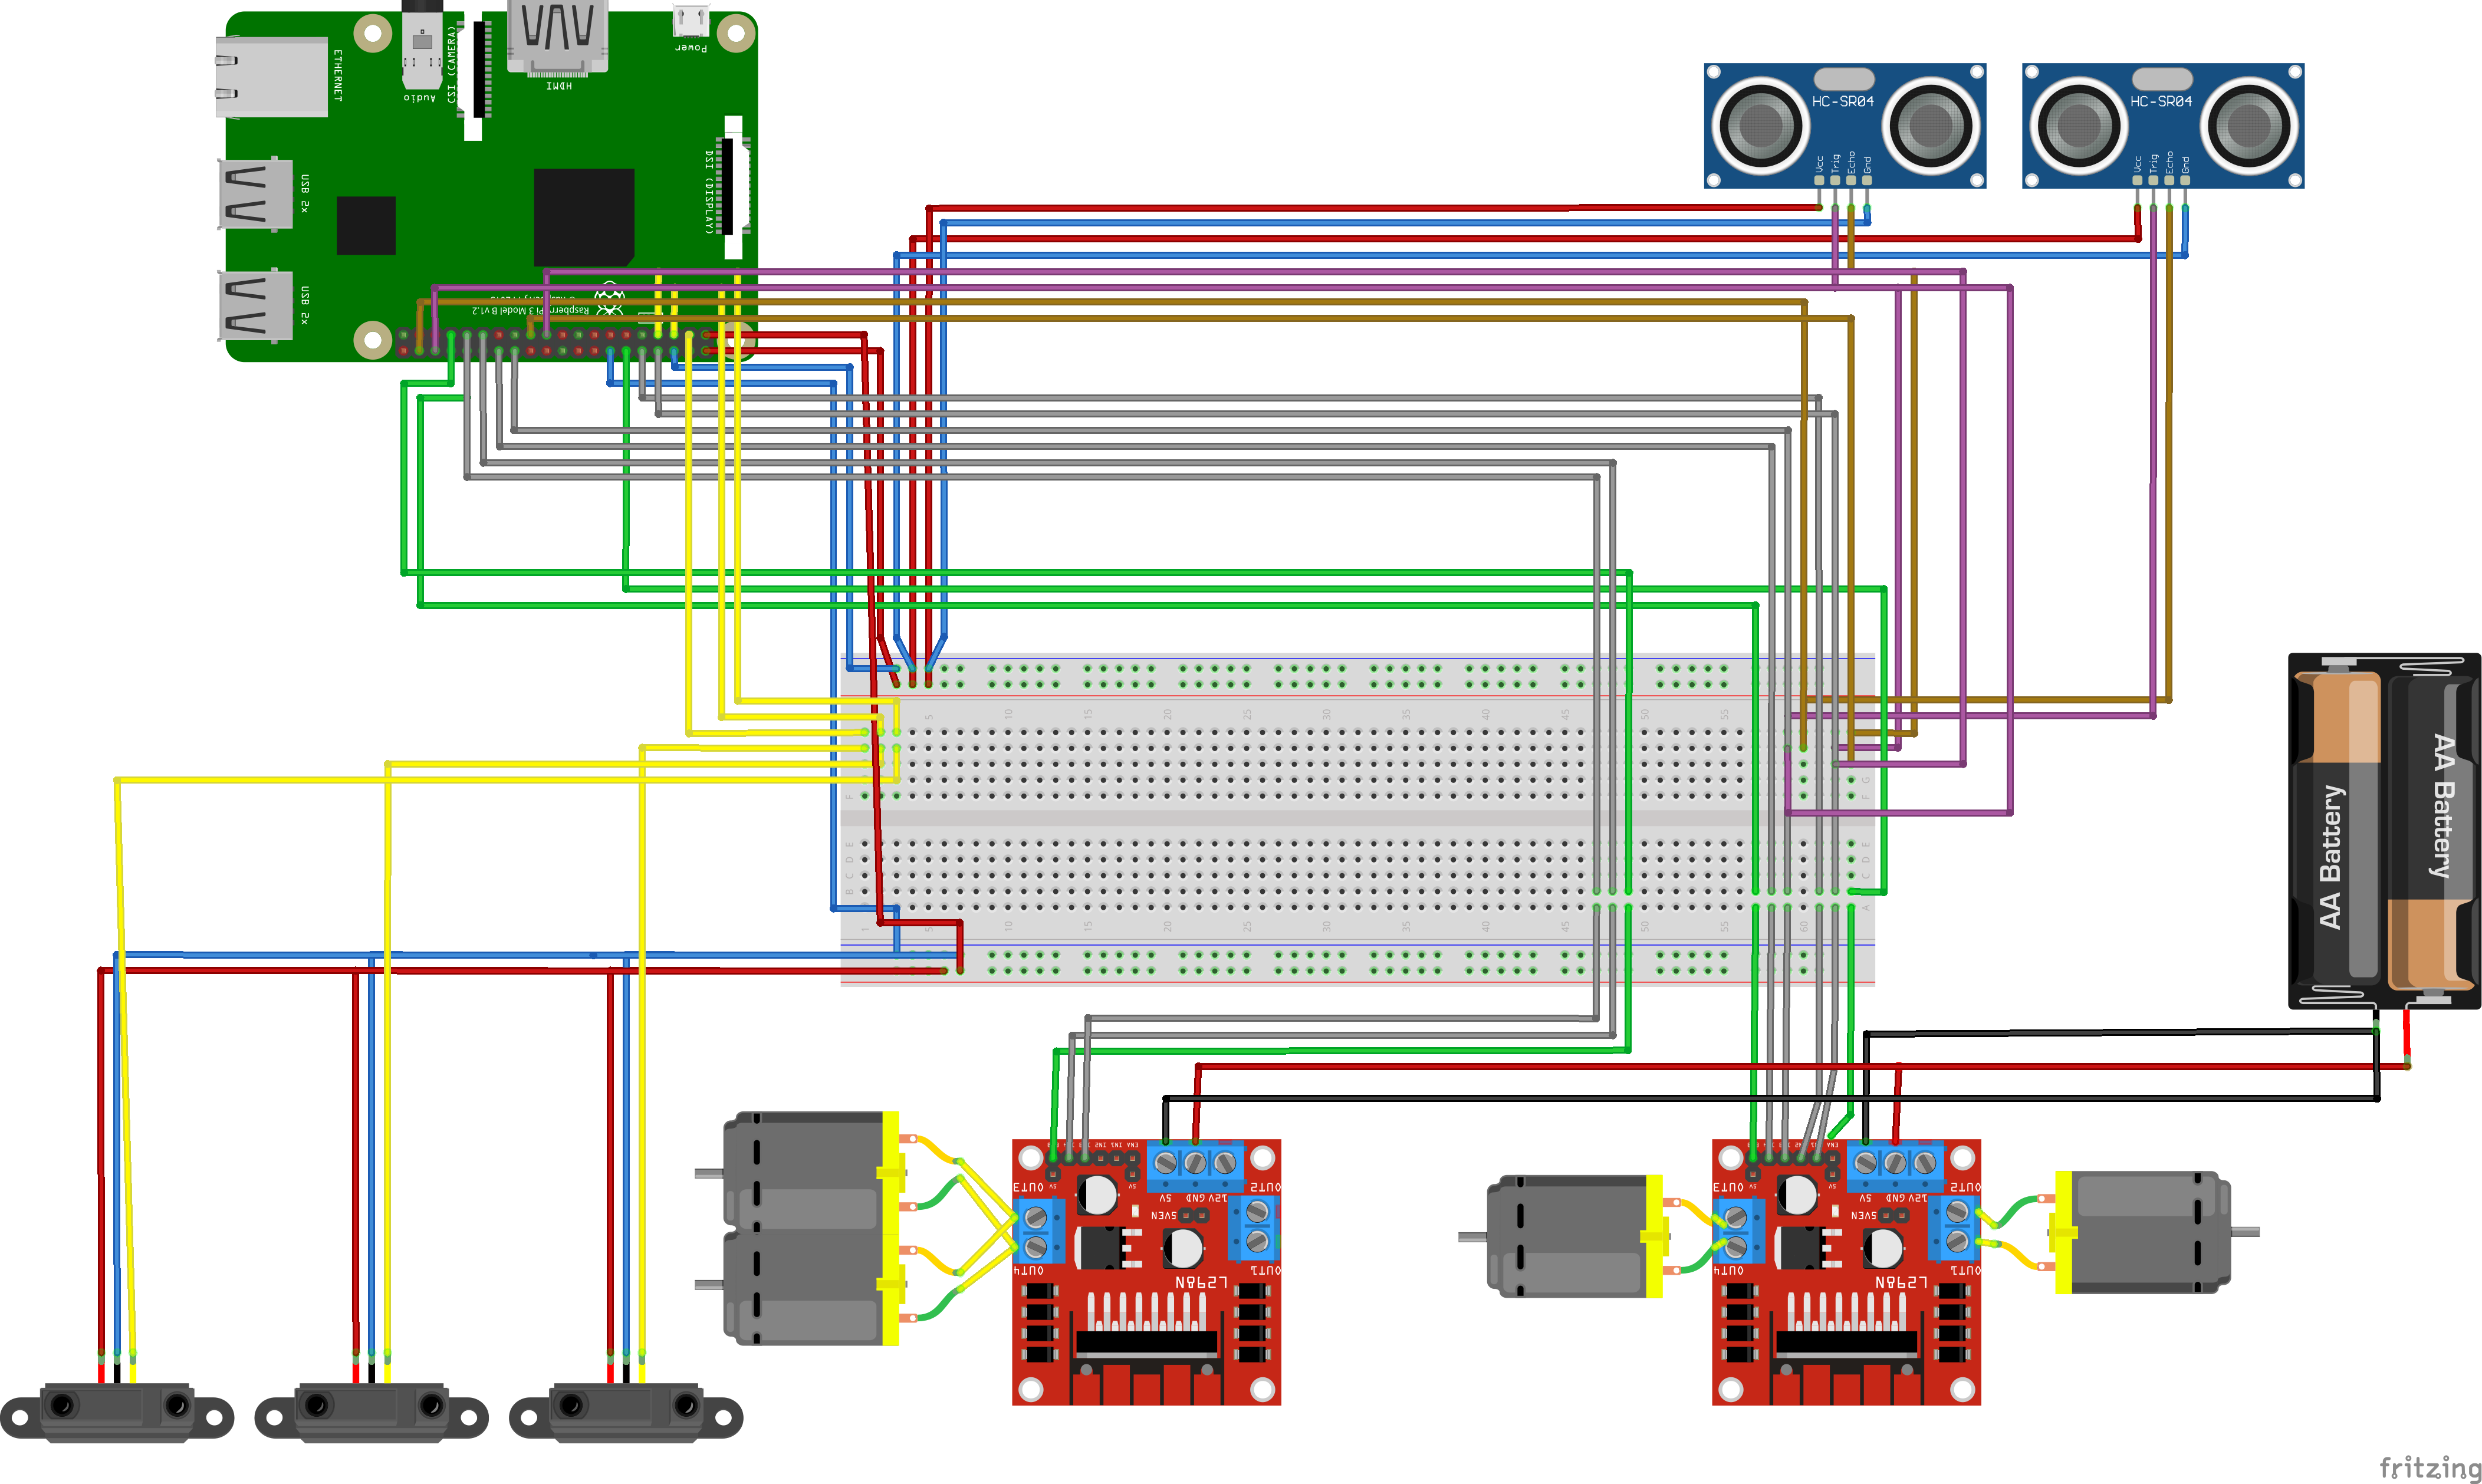
\includegraphics[width=0.98\textheight,height=0.98\textwidth,keepaspectratio,angle=90]{content/assets/Roboter_Steckplatine.png}
\dhbwAppendix{app:object_detection_training_ad}

Aktivitätsdiagram für das Training eines YOLO Modells.

\begin{plantuml}    
@startuml
start
:Bilder aufzeichnen;
:Bilder labeln;
:Bilder in Trainings- und Verifizierungsdaten aufteilen;
:Basismodell auswählen;
repeat
    :Modell konfigurieren;
    :Modell einlernen;
repeat while (Modell funktional?) is (nein)
->ja;
stop
@enduml
\end{plantuml}

\dhbwAppendix{app:actual_objecti_detection_ad}

Aktivitätsdiagram für die Objekterkennung auf dem Raspberry Pi.

\begin{plantuml}
@startuml
start
:Starte separaten Thread;
:Lade YOLO-Modell;
repeat
    :Zeichne Bild auf;
    :Verarbeite Bild;
    while (CPU-Temperatur zu hoch?)
        :Warte;
    endwhile
    
repeat while (Stop Signal?) is (nein)
->ja;
stop
@enduml
\end{plantuml}
\end{dhbwappendices}

\dhbwPrintBibliography

\end{document}
